\documentclass[12pt]{article}
\usepackage[a4paper,
            bindingoffset=0.2in,
            left=1in,
            right=1in,
            top=1in,
            bottom=1in,
            footskip=.25in]{geometry}
\usepackage{amsmath}
\usepackage{amsfonts}
\usepackage{tcolorbox}
\usepackage{cancel}
\usepackage{bbm}
\usepackage{enumitem}
\usepackage{physics}
\usepackage{amssymb}
\usepackage{pgfplots}
\pgfplotsset{width=10cm,compat=1.9}
\usepackage{amsthm}
\usepackage{graphicx}
\newcommand*{\del}{\mathrm{d}}

\newtheorem{proposition}{Proposition}

\title{Simulating Discrete Random Variables with MATLAB}
\author{Evgenii Samutichev}

\begin{document}
\maketitle

\section*{Sampling from a binomial distribution}

\setcounter{equation}{0}

\textbf{Part 1} We have the (pseudo)random number generator for the uniform distribution on $[0,1]$, which is exactly the MATLAB \verb|rand| function. Denote it as $R \sim \text{Unif}(0,1)$. Then, we can transform it to get the random number generator for $X \sim \text{Bern}(p)$ as follows 
\begin{equation}
    X = \mathbbm{1}_{R \leq  p} = \begin{cases}
        1, &R \leq p \\
        0, &R > p
    \end{cases}
\end{equation} 
Then 
\begin{equation}
    \mathbb{P}(X = 1) = \mathbb{P}(R \in [0, p]) =p 
\end{equation}
and 
\begin{equation}
    \mathbb{P}(X = 0) = \mathbb{P}(R \in (p, 1]) = 1 - p
\end{equation}
which proves that $X \sim \text{Bern}(p)$. \textbf{Code:} \verb|bernoulli.m|

\noindent \textbf{Part 2} By fixing $n$, we can also build the random number generator for $Y \sim \text{Binom}(n, p)$ as
\begin{equation}
    Y = X_1 + ... + X_n
\end{equation}
using the definition of Binomial distribution and where $X_i \sim \text{Bern}(p)$. So it's a sum of $n$ samples from $X$. \textbf{Code:} \verb|binomial.m|

\begin{figure}[h!]
    \centering
    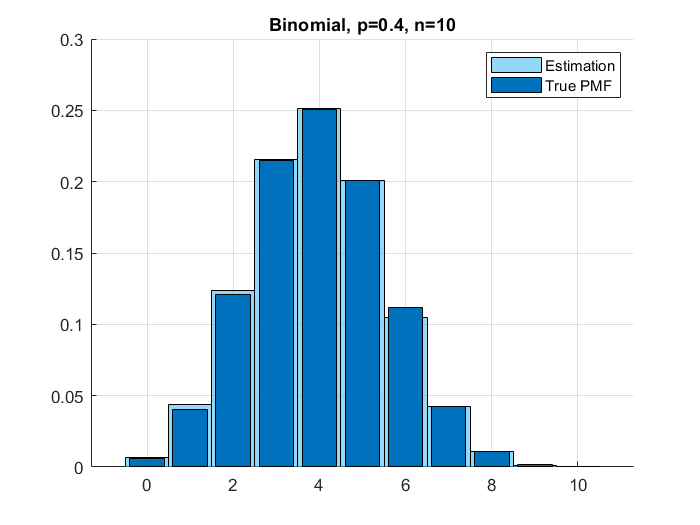
\includegraphics[width=0.6\textwidth]{plot1.png}
\end{figure}

\section*{Sampling from a Poisson distribution}

\setcounter{equation}{0}
\noindent \textbf{Part 1} Let $X \sim \text{Unif}(0, 1)$, then for $Z = -\log X$ we have $Z \geq 0$ and so for $z \geq 0$
\begin{align}
\begin{split}
    F_Z(z) &= \mathbb{P}(Z \leq z) = \mathbb{P}(-\log X \leq z) = \mathbb{P}(e^{-\log X} \leq e^{z}) =\\
    &= \mathbb{P}\left(\frac{1}{X} \leq e^{z}\right) = \mathbb{P}(X \geq e^{-z}) = 1 - e^{-z}
\end{split}
\end{align}
where we can ignore case $X = 0$, since it has zero probability. Including $z < 0$ we get  
\begin{equation}
    F_Z(z) = \begin{cases}
        1 - e^{-z}, &z \geq 0 \\
        0, &z < 0
    \end{cases}
\end{equation}

By taking the derivative of $F_Z$, we get 
\begin{equation}
    f_Z(z) = \frac{dF_Z}{dz} (z) = e^{-z}
\end{equation}
for $z \geq 0$ and $0$ otherwise, which is a density function of $\text{Exp}(1)$, so $Z \sim \text{Exp}(1)$.

\noindent \textbf{Part 2} Now, let's look at the finite sums of i.i.d random variables $Z_i \sim \text{Exp}(1)$. Using the convolution formula for the sum $S_2 = Z_1 + Z_2 \geq 0$, we get
\begin{equation}
    f_{S_2}(z) = \int_{-\infty}^{\infty}{f_{Z}(x) f_Z(z-x) dx} = \int_{0}^{z}{e^{-x}e^{-z+x}dx} = \int_{0}^{z}{e^{-z}dx} = e^{-z} z
\end{equation}

For $S_3 = Z_1 + Z_2 + Z_3 = S_2 + Z_3 \geq 0$ we get 
\begin{align}
\begin{split}
    f_{S_3}(z) &= \int_{-\infty}^{\infty}{f_{S_2}(x) f_Z(z-x) dx} = \int_{0}^{z}{e^{-x} x e^{-z+x}dx} = \\
    &=  e^{-z} \int_{0}^{z}{ x dx} = \frac{e^{-z} z^2}{2}
\end{split}
\end{align}

It's now tempting to assume that the general form is 
\begin{equation}
    f_{S_k}(z) = \frac{e^{-z} z^{k-1}}{(k-1)!}
\end{equation}
let's prove this by induction. If it's true for $k$, then for $k+1$
\begin{align}
    \begin{split}
    f_{S_{k+1}}(z) &= \int_{-\infty}^{+\infty}{f_{S_k}(x) f_{Z}(z-x) dx} = \int_{0}^{z}{e^{-x}\frac{x^{k-1}}{(k-1)!}e^{-z+x} dx} = \\
    &= \frac{e^{-z}}{(k-1)!} \int_{0}^{z}{x^{k-1} dx} = \frac{e^{-z}}{(k-1)!} \frac{z^k}{k} =  \frac{e^{-z}z^{k}}{k!}
    \end{split}
\end{align}
so by induction this is true for all $k$ and $S_k \sim \text{Gamma}(k, 1)$

\noindent \textbf{Part 3} Let $\lambda > 0$ and let $(X_n)_{n \geq 0}$ be a sequence of i.i.d as $X \sim \text{Unif}(0,1)$ r.v.s. Then let $Y$ be a random variable defined as 
\begin{equation}
    Y = \min\{n \geq 0 | X_0 \cdot ... \cdot X_n \leq e^{-\lambda}\}
\end{equation}

Notice that the event 
\begin{equation}
    X_0 \cdot ... \cdot X_n \leq e^{-\lambda}
\end{equation}
is equivalent to 
\begin{equation}
    \sum_{k=0}^{n}{\log X_k} = \log (X_0 \cdot ... \cdot X_n) \leq \log(e^{-\lambda}) = -\lambda 
\end{equation}
and event $(X_0 = 0) \cup (X_1 = 0) \cup ... \cup (X_n = 0)$ has probability zero, so we can ignore it. Multiplying both sides by $-1$ we get 
\begin{equation}
    \sum_{k=0}^{n}{-\log X_k} = \sum_{k=0}^{n}{Z_k} = S_{k+1} \geq \lambda
\end{equation}
where we used result of \textbf{Part 1} of this problem. Then 
\begin{equation}
    (Y = 0) = (S_1 \geq \lambda)
\end{equation}
and for $n > 0$
\begin{equation}\label{eq:1}
    (Y=n) = (S_{n+1} \geq \lambda ) \setminus (S_n \geq \lambda)
\end{equation}


From \textbf{Part 2} we get 
\begin{equation}
    \mathbb{P}(S_{n+1} \geq \lambda) = \int_{\lambda}^{\infty}{\frac{e^{-x}x^{n}}{n!} dx}
\end{equation} 

We can now compute the PMF of $Y$. First, notice that 
\begin{equation}
    \mathbb{P}(Y = 0) =\int_{\lambda}^{\infty}{e^{-x} dx} = -e^{-x} \Big|_{\lambda}^{\infty} = e^{-\lambda} = \frac{\lambda^0}{0!}e^{-\lambda}
\end{equation}
so the formula holds for $n= 0$. For $n > 0$ 
\begin{align}
\begin{split}
    \mathbb{P}(S_{n+1} \geq \lambda)&= \int_{\lambda}^{\infty}{\frac{e^{-x}x^{n}}{n!} dx} = - e^{-x} \frac{x^{n}}{n!} \Big|_{\lambda}^{\infty} +\int_{\lambda}^{\infty}{\frac{e^{-x}x^{n-1}}{(n-1)!} dx} = \\
    &= e^{-\lambda} \frac{\lambda^n}{n!} + \mathbb{P}(S_{n} \geq \lambda)
\end{split}
\end{align}
then using \eqref{eq:1}
\begin{equation}
    \mathbb{P}(Y = n) = \mathbb{P}(S_{n+1} \geq \lambda) - \mathbb{P}(S_{n} \geq \lambda) = e^{-\lambda} \frac{\lambda^n}{n!} 
\end{equation}

So indeed $Y \sim \text{Pois}(\lambda)$.

\noindent \textbf{Part 4} For the algorithm see \verb|poisson.m|, it's vectorized to avoid for loops as much as possible.

\begin{figure}[h!]
    \centering
    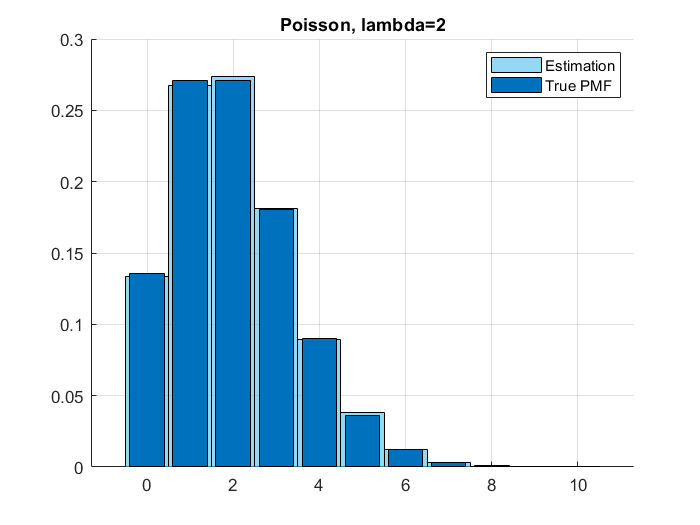
\includegraphics[width=0.6\textwidth]{plot2.png}
\end{figure}

\newpage
\section*{The inversion method}
\setcounter{equation}{0}

\textbf{Part 1} Let $P = (p_0, p_1, ..., )$ be a probability distribution on $\mathbb{N}$. Let $H : \mathbb{R} \to [0, 1]$ be a function defined as 
\begin{equation}
    \forall k \geq 0, \forall x \in [k, k+1) \text{ then } H(x) = p_0 + p_1 + ... + p_k
\end{equation}
and let $U \sim \text{Unif}(0, 1)$. Define $X$ as 
\begin{equation}
    X = \inf \{k \in \mathbb{N} \ | \ U \leq  H(k)\}
\end{equation}
then 
\begin{equation}
    \mathbb{P}(X=0) = \mathbb{P}(U \leq p_0) = p_0
\end{equation}
and notice that for $n > 0$
\begin{equation}
    (X = n) = (U \leq H(n)) \setminus (U \leq H(n-1))
\end{equation}
since $H(x)$ is a nondecreasing function, so if $n$ is an infimum, then for smaller value as $n-1$ the inequality $U \leq H(n-1)$ can't hold. Then 
\begin{equation}
    \mathbb{P}(X=n) = \mathbb{P}(U \leq H(n)) - \mathbb{P}(U \leq H(n-1)) = \sum_{k=0}^{n}{p_k} - \sum_{k=0}^{n-1}{p_k} = p_n
\end{equation}

\noindent \textbf{Part 2} The result of \textbf{Part 1} allows us to sample from any discrete distribution. In particular, let's sample from geometric distribution with parameter $p$. For an algorithm see \verb|geometric.m|.

\begin{figure}[h!]
    \centering
    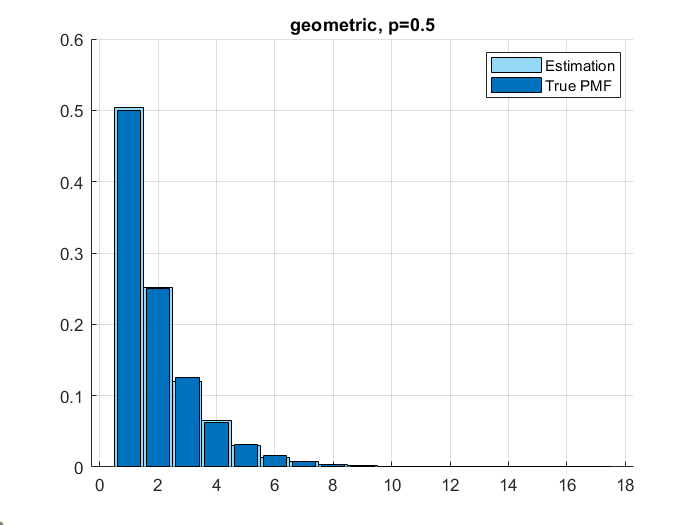
\includegraphics[width=0.6\textwidth]{plot3.png}
\end{figure}
\end{document}